\begin{frame}
  \frametitle{\textbf{Kinematics in Particle Detectors}}
  \begin{columns}
    \column{0.4\textwidth}
    \centering
    \newcommand \px {0.6}
    \newcommand \py {1.3}
    \newcommand \pz {0.8}
    \begin{tikzpicture}
      \tdplotsetmaincoords{70}{110}
      \draw[->] (0,0,0) to (xyz cylindrical cs:radius=2) node[anchor=north west]{$z$};
      \draw[->] (0,0,0) to (xyz cylindrical cs:radius=1.5,angle=90) node[anchor=south]{$x$};
      \draw[->] (0,0,0) to (xyz cylindrical cs:z=3) node[anchor=east]{$y$};
      \node[cylinder, draw, shape aspect=1, minimum height = 2cm, minimum width = 1.2cm] {};
      \draw[->,color=red,thick] (0,0,0) to (\px,\py,\pz) node[color=red,thick,anchor=south]{$\vec{p}$};
      \draw[-,color=gray] (0,0,0) to (0.0,\py,\pz);
      %\draw[-,color=gray] (0,0,0) to (\px,\py,0.0);
      %\draw[-,dashed,color=gray] (\px,\py,\pz) to (\px,\py,0.0);
      \draw[-,dashed,color=gray] (\px,\py,\pz) to (0.0,\py,\pz);
      \draw[-,dashed,color=gray] (0.0,\py,0.0) to (0.0,\py,\pz);
      %\draw[-,dashed,color=gray] (0.0,\py,0.0) to (\px,\py,0.0);
      \draw[->] (.3,0,0) arc [start angle=0,end angle=60,x radius=0.4,y radius=0.3] node[anchor=west]{$\text{  }\theta$};
      \draw[->] (0,1.2,0) arc [start angle=90,end angle=160,x radius=0.25,y radius=0.5] node[anchor=south east]{\ $\phi$};
      \node[font=\tiny] at (0.7,-0.76) {detector};
      \node[font=\tiny] at (1.65,0.2) {beam axis};
      %\node[font=\scriptsize] at (-1,2) {\textbf{Detector geometry}};
    \end{tikzpicture}

    \

    \begin{tikzpicture}
      \node{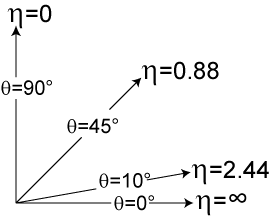
\includegraphics[width=0.58\textwidth]{Pseudorapidity2.png}};
      \node[font=\tiny] at (0,-1.3) {\href{https://en.wikipedia.org/wiki/Pseudorapidity}{fig. ref.}};
    \end{tikzpicture}
    \column{0.6\textwidth}
    \begin{itemize}
    \item Detector geometry warrants the use of cylindrical coordinate system
    \end{itemize}
    \begin{align*}
      \text{transverse momentum} : p_{\text{T}} &= \left|\vec{p}\right| \sin\theta \\
      \text{rapidity} : y &= \cfrac{1}{2} \ln \left( \cfrac{E + p_z}{E - p_z} \right)
      \\
      \text{psuedo-rapidity} :\eta &= \cfrac{1}{2} \ln \left( \cfrac{p + p_z}{p - p_z} \right) \\
      & \to -\ln \left[ \tan\left(\cfrac{\theta}{2}\right) \right]
    \end{align*}
    \begin{itemize}
    \item Why are these variables common in particle physics experiments?
      \begin{itemize}
      \item $\sum_{i} p_{\text{T},i} = 0 + \epsilon$
      \item $\Delta y$ is invariant for boosts along $z$-axis
      \end{itemize}
    \end{itemize}
  \end{columns}
  
  
\end{frame}
